%Version 3 December 2023
% See section 11 of the User Manual for version history
%
%%%%%%%%%%%%%%%%%%%%%%%%%%%%%%%%%%%%%%%%%%%%%%%%%%%%%%%%%%%%%%%%%%%%%%
%%                                                                 %%
%% Please do not use \input{...} to include other tex files.       %%
%% Submit your LaTeX manuscript as one .tex document.              %%
%%                                                                 %%
%% All additional figures and files should be attached             %%
%% separately and not embedded in the \TeX\ document itself.       %%
%%                                                                 %%
%%%%%%%%%%%%%%%%%%%%%%%%%%%%%%%%%%%%%%%%%%%%%%%%%%%%%%%%%%%%%%%%%%%%%

%%\documentclass[referee,sn-basic]{sn-jnl}% referee option is meant for double line spacing

%%=======================================================%%
%% to print line numbers in the margin use lineno option %%
%%=======================================================%%

%%\documentclass[lineno,sn-basic]{sn-jnl}% Basic Springer Nature Reference Style/Chemistry Reference Style

%%======================================================%%
%% to compile with pdflatex/xelatex use pdflatex option %%
%%======================================================%%

%%\documentclass[pdflatex,sn-basic]{sn-jnl}% Basic Springer Nature Reference Style/Chemistry Reference Style


%%Note: the following reference styles support Namedate and Numbered referencing. By default the style follows the most common style. To switch between the options you can add or remove “Numbered” in the optional parenthesis. 
%%The option is available for: sn-basic.bst, sn-vancouver.bst, sn-chicago.bst%  
 
%%\documentclass[pdflatex,sn-nature]{sn-jnl}% Style for submissions to Nature Portfolio journals
%%\documentclass[pdflatex,sn-basic]{sn-jnl}% Basic Springer Nature Reference Style/Chemistry Reference Style
\documentclass[pdflatex,sn-mathphys-num]{sn-jnl}% Math and Physical Sciences Numbered Reference Style 
%%\documentclass[pdflatex,sn-mathphys-ay]{sn-jnl}% Math and Physical Sciences Author Year Reference Style
%%\documentclass[pdflatex,sn-aps]{sn-jnl}% American Physical Society (APS) Reference Style
%%\documentclass[pdflatex,sn-vancouver,Numbered]{sn-jnl}% Vancouver Reference Style
%%\documentclass[pdflatex,sn-apa]{sn-jnl}% APA Reference Style 
%%\documentclass[pdflatex,sn-chicago]{sn-jnl}% Chicago-based Humanities Reference Style

%%%% Standard Packages
%%<additional latex packages if required can be included here>

\usepackage{graphicx}%
\usepackage{multirow}%
\usepackage{amsmath,amssymb,amsfonts}%
\usepackage{amsthm}%
\usepackage{mathrsfs}%
\usepackage[title]{appendix}%
\usepackage{xcolor}%
\usepackage{textcomp}%
\usepackage{manyfoot}%
\usepackage{booktabs}%
\usepackage{algorithm}%
\usepackage{algorithmicx}%
\usepackage{algpseudocode}%
\usepackage{listings}%
\usepackage{float}
%%%%

%%%%%=============================================================================%%%%
%%%%  Remarks: This template is provided to aid authors with the preparation
%%%%  of original research articles intended for submission to journals published 
%%%%  by Springer Nature. The guidance has been prepared in partnership with 
%%%%  production teams to conform to Springer Nature technical requirements. 
%%%%  Editorial and presentation requirements differ among journal portfolios and 
%%%%  research disciplines. You may find sections in this template are irrelevant 
%%%%  to your work and are empowered to omit any such section if allowed by the 
%%%%  journal you intend to submit to. The submission guidelines and policies 
%%%%  of the journal take precedence. A detailed User Manual is available in the 
%%%%  template package for technical guidance.
%%%%%=============================================================================%%%%

%% as per the requirement new theorem styles can be included as shown below
\theoremstyle{thmstyleone}%
\newtheorem{theorem}{Theorem}%  meant for continuous numbers
%%\newtheorem{theorem}{Theorem}[section]% meant for sectionwise numbers
%% optional argument [theorem] produces theorem numbering sequence instead of independent numbers for Proposition
\newtheorem{proposition}[theorem]{Proposition}% 
%%\newtheorem{proposition}{Proposition}% to get separate numbers for theorem and proposition etc.

\theoremstyle{thmstyletwo}%
\newtheorem{example}{Example}%
\newtheorem{remark}{Remark}%

\theoremstyle{thmstylethree}%
\newtheorem{definition}{Definition}%

\raggedbottom
%%\unnumbered% uncomment this for unnumbered level heads

\begin{document}

\title[Article Title]{LLMBot: Multi-Agent Robotic Systems for Adaptive Task Execution}

%%=============================================================%%
%% GivenName	-> \fnm{Joergen W.}
%% Particle	-> \spfx{van der} -> surname prefix
%% FamilyName	-> \sur{Ploeg}
%% Suffix	-> \sfx{IV}
%% \author*[1,2]{\fnm{Joergen W.} \spfx{van der} \sur{Ploeg} 
%%  \sfx{IV}}\email{iauthor@gmail.com}
%%=============================================================%%


\author{\fnm{Harith} \sur{Ibrahim}}\email{harithsami01@gmail.com}
\author{\fnm{Shane} \sur{Xi}}\email{S.Q.Xie@leeds.ac.uk}

\author{\fnm{Harith} \sur{Alsafi}}\email{harith.alsafi@gmail.com}



\affil{\orgdiv{School of Computing}, \orgname{University of Leeds}, \orgaddress{\street{Street}, \city{Leeds}, \postcode{LS2 9JT}, \state{West Yorkshire}, \country{United Kingdom}}}


%%==================================%%
%% Sample for unstructured abstract %%
%%==================================%%

\abstract{Robotic task planning systems often require significant computational resources and financial investment, limiting their accessibility and scalability. Can we leverage recent advancements in Large Language Models (LLMs) to create more cost-effective and lightweight robotic planning solutions? This paper introduces an innovative framework that integrates LLMs with robotic systems for natural language interaction and task execution. Our approach, which we call LLMRP (Large Language Model Robotic Planner), combines GPT-3.5 Turbo for natural language understanding, reasoning, and high-level task planning with a simulated 3D environment in Unreal Engine. LLMRP uses behavior trees for robust low-level execution of robotic actions, grounding the LLM's capabilities in a practical robotic context. The system employs prompt engineering, multimodal input, and parameter optimization to enhance the LLM's performance and reduce computational overhead. For systematic evaluations, we developed a comprehensive test suite assessing success rates, spatial distributions, and cost-effectiveness across various scenarios. Experimental results demonstrate that our approach outperforms traditional planning systems in terms of computational efficiency and cost-effectiveness while maintaining comparable task success rates. Additionally, we have demonstrated LLMRP using a simulated mobile manipulator in Unreal Engine. This research advances multi-agent collaboration and human-robot interaction by enabling more intuitive and resource-efficient communication between humans and robots. By combining modern language models with lightweight execution frameworks, this project paves the way for more accessible, adaptive, and cost-effective robotic solutions capable of natural language-based collaboration.}

%%================================%%
%% Sample for structured abstract %%
%%================================%%
 
% \abstract{\textbf{Purpose:} The abstract serves both as a general introduction to the topic and as a brief, non-technical summary of the main results and their implications. The abstract must not include subheadings (unless expressly permitted in the journal's Instructions to Authors), equations or citations. As a guide the abstract should not exceed 200 words. Most journals do not set a hard limit however authors are advised to check the author instructions for the journal they are submitting to.
% 
% \textbf{Methods:} The abstract serves both as a general introduction to the topic and as a brief, non-technical summary of the main results and their implications. The abstract must not include subheadings (unless expressly permitted in the journal's Instructions to Authors), equations or citations. As a guide the abstract should not exceed 200 words. Most journals do not set a hard limit however authors are advised to check the author instructions for the journal they are submitting to.
% 
% \textbf{Results:} The abstract serves both as a general introduction to the topic and as a brief, non-technical summary of the main results and their implications. The abstract must not include subheadings (unless expressly permitted in the journal's Instructions to Authors), equations or citations. As a guide the abstract should not exceed 200 words. Most journals do not set a hard limit however authors are advised to check the author instructions for the journal they are submitting to.
% 
% \textbf{Conclusion:} The abstract serves both as a general introduction to the topic and as a brief, non-technical summary of the main results and their implications. The abstract must not include subheadings (unless expressly permitted in the journal's Instructions to Authors), equations or citations. As a guide the abstract should not exceed 200 words. Most journals do not set a hard limit however authors are advised to check the author instructions for the journal they are submitting to.}

\keywords{Large Language Models, Robotic Systems, Natural Language Interaction, Task Planning, Human-Robot Interaction, Multi-agent Collaboration, Warehouse Automation, Behavior Trees, Simulated Environment, Physical Task Execution, Embodiment}

%%\pacs[JEL Classification]{D8, H51}

%%\pacs[MSC Classification]{35A01, 65L10, 65L12, 65L20, 65L70}
\maketitle


\section{Introduction}\label{sec1}
Effective robotic task planning requires not only a deep understanding of the environment and available actions but also the ability to interpret and execute high-level, natural language instructions. Traditional approaches to robot planning often involve complex, expensive algorithms that are difficult to develop and maintain. Can we leverage recent advancements in large language models (LLMs) to create more accessible and cost-effective robot planning solutions? Our work introduces LLM-RP (Large Language Model Robotic Planner), a novel framework that integrates LLMs with symbolic planning methods for intuitive, natural language-based robot control.

LLMs trained on vast corpora of text have demonstrated remarkable multi-task generalization and common-sense reasoning capabilities. Recent research has explored their potential in robotic task planning by generating or scoring action sequences. However, these approaches often lack grounding in the robot's physical capabilities and current environmental state. LLM-RP addresses this limitation by combining the rich language understanding of LLMs with the efficiency and adaptability of symbolic planners, specifically behavior trees.
\begin{figure}[h]
\centering
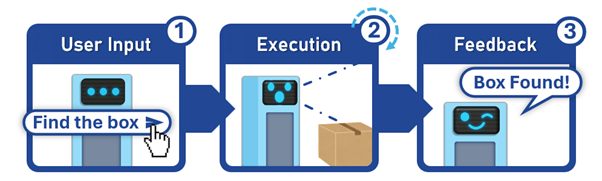
\includegraphics[width=0.7\textwidth]{figures/Picture13.png}
\caption{Diagram Showing Simplified Project Plan}\label{fig1}
\end{figure}
A key component of LLM-RP is its use of GPT-3.5 Turbo for natural language understanding, reasoning, and high-level task planning. We leverage the fact that LLMs are trained on diverse web content, including programming tutorials and documentation, to create a novel prompting scheme. This scheme provides the LLM with a Pythonic-style program structure, including available actions, environment objects, and function definitions for tasks. We incorporate situated awareness by asserting preconditions and implementing recovery actions for failed assertions.

LLM-RP operates within a simulated 3D environment in Unreal Engine, allowing for comprehensive testing and evaluation. The system utilizes behavior trees for robust low-level execution of robotic actions, bridging the gap between high-level language understanding and concrete robot behaviors. We employ prompt engineering, multimodal input, and parameter optimization to enhance the LLM's performance and reduce computational overhead.


Our approach goes beyond simple language-to-action mapping. LLM-RP enables robots to interpret complex, free-form natural language instructions, reason about the given task, and coherently execute the necessary actions to accomplish the objective. Moreover, it exhibits adaptability to handle novel situations without extensive retraining or reprogramming.

To evaluate LLM-RP, we developed a comprehensive test suite assessing success rates, spatial distributions, and cost-effectiveness across various scenarios. Our results demonstrate that LLM-RP outperforms traditional planning systems in terms of computational efficiency and cost-effectiveness while maintaining comparable task success rates. We also showcase LLM-RP's capabilities using a simulated mobile manipulator in Unreal Engine, highlighting its potential for real-world applications.

This research advances multi-agent collaboration and human-robot interaction by enabling more intuitive and resource-efficient communication between humans and robots. By combining modern language models with lightweight execution frameworks, LLM-RP paves the way for more accessible, adaptive, and cost-effective robotic solutions capable of natural language-based collaboration.

\section{Background and related work}

\subsection{Task Planning in Robotics}

Traditional approaches to robotic task planning often involve search algorithms within pre-defined domains (Fikes and Nilsson, 1971; Jiang et al., 2018; Garrett et al., 2020). These methods can be computationally expensive and challenging to scale in environments with numerous feasible actions and objects (Puig et al., 2018; Shridhar et al., 2020). To address this, researchers have explored various techniques, including heuristic-guided search (Baier et al., 2007; Hoffmann, 2001; Helmert, 2006) and learning-based task and motion planning (Akakzia et al., 2021; Eysenbach et al., 2019; Jiang et al., 2019).

Our approach, LLM-RP, takes a different route by leveraging large language models to directly generate plans that include conditional reasoning and error correction, bypassing the need for extensive search.

\subsection{Large Language Models and Conversational Tuning}

Large Language Models (LLMs) like GPT-3 are neural networks trained on vast amounts of text data, enabling them to generate human-like text outputs. Their training process exposes them to a wide range of knowledge and scenarios, allowing them to exhibit reasoning, common sense, and goal-oriented behaviors. Recent work has explored the use of LLMs in robotic task planning (Ahn et al., 2022; Huang et al., 2022a, b; Li et al., 2022), but challenges remain in bridging the gap between language understanding and executable robot actions.

LLM-RP builds upon these advances by integrating GPT-3.5 Turbo for natural language understanding and high-level planning, while addressing the grounding problem through a novel prompting scheme and integration with symbolic planners.

\subsection{Embodied Large Language Models}

Recent research has explored techniques to enhance LLMs' capabilities for embodied environments like robotics, including prompt engineering, multimodal prompting, and few-shot learning. These techniques leverage language to define the rules of the world and the robot's abilities, a process called "grounding" (Huang et al., 2022b; Ahn et al., 2022).

Our work extends this concept by introducing a programming language-inspired prompting scheme that informs the LLM of both the situated environment state and available robot actions, ensuring output compatibility with robot capabilities.

\subsection{Symbolic Planning Methods}

Symbolic planning techniques, such as behavior trees, offer a simple yet powerful way to create adaptable logic and decision-making without the need for complex machine learning models. While recent works have explored learning-based approaches to task planning (Mirchandani et al., 2021; Nair and Finn, 2020; Shah et al., 2022), these methods often struggle with generalization to novel situations.

LLM-RP combines behavior trees with LLMs, leveraging the strengths of both components: LLMs provide rich language understanding capabilities, while symbolic planners offer computational efficiency and the ability to rapidly re-plan lower-level actions based on changes to the symbolic world state.

\subsection{Cost-Effective Robotic Planning}

A key challenge in robotic task planning is the development of sophisticated algorithms that are both effective and cost-efficient. Traditional approaches often require significant computational resources and financial investment, limiting their accessibility and scalability.

Our work addresses this challenge by proposing a lightweight, LLM-integrated approach that reduces computational overhead while maintaining high task success rates. By leveraging the pre-trained knowledge of LLMs and combining it with efficient symbolic planning methods, LLM-RP aims to provide a more accessible and cost-effective solution for robotic task planning.

\subsection{Simulated Environments for Robotic Research}

Simulated environments play a crucial role in robotics research, allowing for rapid prototyping, testing, and evaluation of algorithms without the need for physical hardware. Recent works have utilized game engines and physics simulators for robotic task planning and learning (Shah et al., 2018; Savva et al., 2019).

LLM-RP operates within a simulated 3D environment in Unreal Engine, enabling comprehensive testing and evaluation of our approach across diverse scenarios. This setup allows us to assess the system's performance, running costs, and cost-effectiveness in a controlled yet realistic setting.



\section{Method}
We use the capabilities of large language models (LLMs) combined with behavior trees to create an intelligent robotic system capable of understanding natural language instructions and performing complex tasks in a simulated environment. Below, we describe how we integrate LLMs with behavior trees, implement robot abilities, and deploy the approach in a virtual Unreal Engine environment for household and industrial scenarios.

\subsection{Integration of Language Models and Behavior Trees}
Our system leverages GPT-3.5 Turbo, a state-of-the-art LLM, for natural language understanding and high-level task planning. We combine this with behavior trees to create a flexible and powerful decision-making framework for robotic agents. Specifically, the LLM:

(i) interprets natural language instructions and converts them into high-level plans

(ii) generates conditional reasoning and error correction strategies

(iii) grounds language understanding in the current environmental context

\begin{figure}[H]
\centering
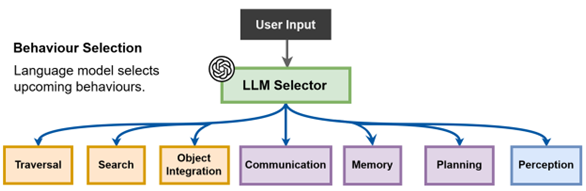
\includegraphics[width=0.6\textwidth]{figures/Picture12.png}
\caption{Proposed approach of utilizing Language Models in Behaviour Trees.}\label{fig7}
\end{figure}
Following recent work (Huang et al., 2022b; Ahn et al., 2022), we use prompting techniques such as zero-shot and few-shot learning, chain of thought reasoning, and multimodal prompting to enhance the model's performance. The behavior trees provide a hierarchical and modular structure for representing complex behaviors, making them easy to design, debug, and maintain.
\subsection{Robot Abilities and Communication}
Our system implements robotic agents, called HelperBots, capable of navigating a virtual environment, interacting with objects, and performing various tasks based on natural language instructions. The HelperBots use five high-level behaviors:

"Go to" for navigation
"Object interact" for manipulating objects
"Refer to memory" for storing and retrieving environmental information
"Status" for reporting internal status
"Communicate" for inter-agent communication

For perception, we assume perfect object identification within the robot's line of vision. Navigation utilizes Unreal Engine's AI navigation system, employing a Navigation Mesh (NavMesh) for efficient pathfinding in the 3D environment.
The system employs context-aware memory within the language model and object memory on the robot logic side. A "Master Robot" serves as a central control unit, with access to the combined memory of all other robots. This hierarchical architecture allows for efficient coordination and task allocation among specialized robots.

\begin{figure}[H]
\centering
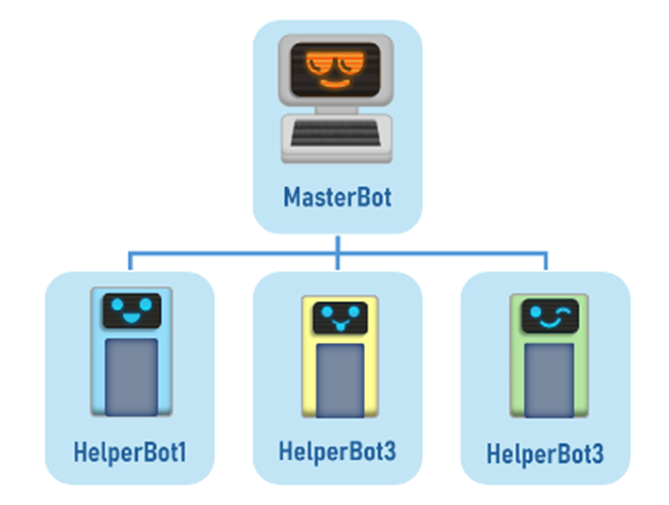
\includegraphics[width=0.5\textwidth]{figures/Picture6.png}
\caption{Diagram of robot command and memory hierarchy.}\label{fig9}
\end{figure}


\subsection{Virtual Environment Implementation}
Given the integrated LLM and behavior tree framework, we implement this system in a virtual Unreal Engine environment simulating both household and industrial scenarios. To do so, we use a Python environment to handle the LLM's logic and reasoning capabilities, which communicates with the Unreal Engine simulation via an API.
\begin{figure}[H]
\centering
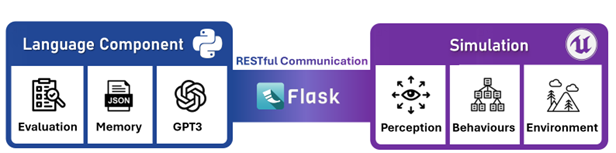
\includegraphics[width=0.7\textwidth]{figures/Picture2.png}
\caption{High level diagram of system architecture.}\label{fig3}
\end{figure}
Receive natural language instructions
Use the LLM to interpret the instructions and generate a high-level plan
Translate the plan into a behavior tree structure
Execute the behavior tree in the simulated environment
Use LLM-generated strategies for error correction and handling unexpected situations

The Unreal Engine environment provides a realistic testbed for our approach, leveraging its strengths in intelligent agent creation, behavior simulation, navigation, and perception systems.
Our approach enhances human-robot interactions by enabling robots to display appropriate emotional expressions based on the chat context. The system's modularity is emphasized through a JSON file configuration system, allowing for easy component replacement without modifying the underlying code.
This implementation allows us to test and evaluate our approach across diverse scenarios, assessing the system's performance in both household and industrial settings. The combination of LLMs and behavior trees provides a flexible and powerful framework for robotic task planning and execution, bridging the gap between natural language understanding and executable robot actions.


% \begin{figure}[h]
% \centering
% 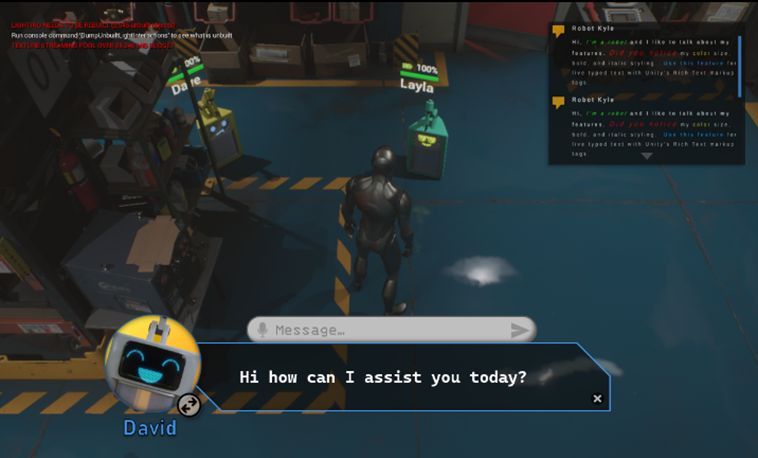
\includegraphics[width=0.6\textwidth]{figures/Picture9.png}
% \caption{Screenshot showing Robot Chat User Interface.}\label{fig4}
% \end{figure}
% \begin{figure}[h]
% \centering
% 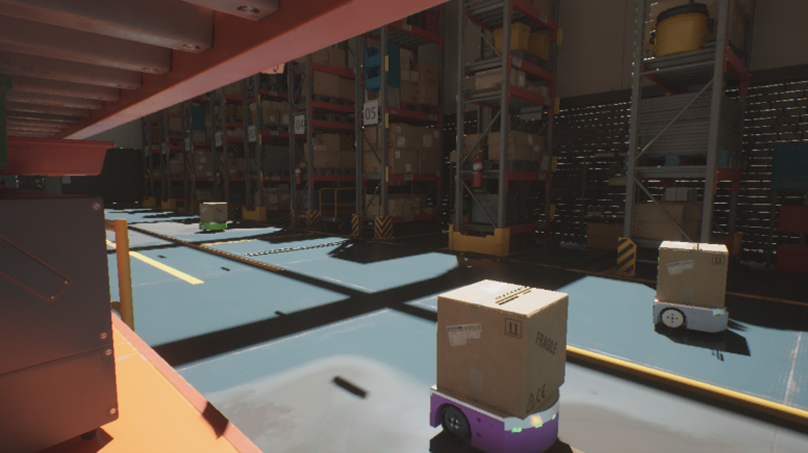
\includegraphics[width=0.6\textwidth]{figures/Picture10.png}
% \caption{Screenshot of the simulation. Intelligent robots managing inventory in a Warehouse.}\label{fig5}
% \end{figure}
% \begin{figure}[H]
% \centering
% 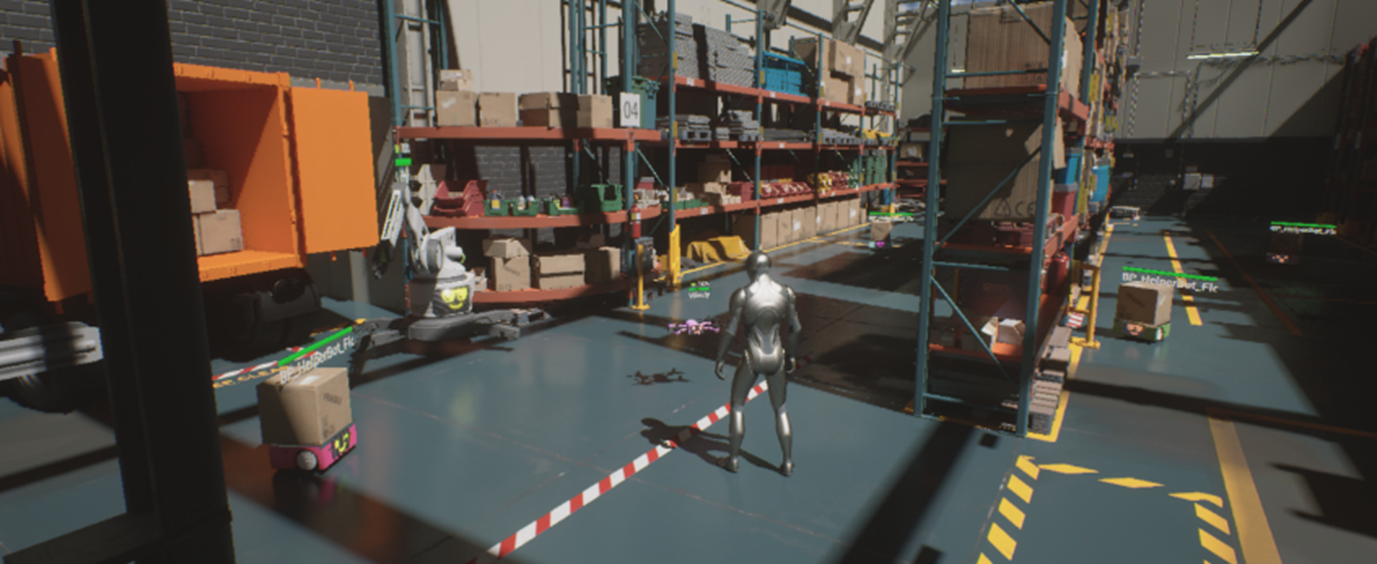
\includegraphics[width=0.6\textwidth]{figures/Picture14.png}
% \caption{Warehouse Simulation Environment in Unreal Engine 5.}\label{fig6}
% \end{figure}
% \begin{figure}[h]
% \centering
% 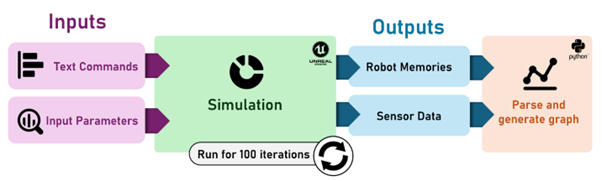
\includegraphics[width=0.8\textwidth]{figures/Picture4.png}
% \caption{Simulation Evaluation process diagram.}\label{fig10}
% \end{figure}
% \begin{figure}[h]
% \centering
% 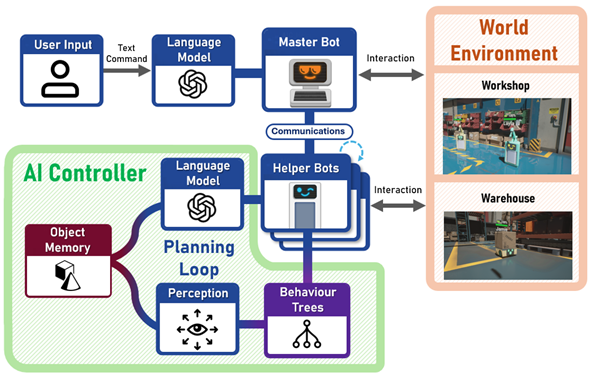
\includegraphics[width=0.9\textwidth]{figures/Picture5.png}
% \caption{Proposed Robot Cognitive Architecture.}\label{fig8}
% \end{figure}

You can simplify and split the algorithm for better readability. Here’s a proposed version with simplifications and the split:

Algorithm: Integrated Cognitive Architecture for LLM-Driven Robotic NPC with Concurrent Perception

Main Execution Loop
\begin{algorithm}
\caption{Main Execution Loop}\label{algo_main_execution_loop}
\begin{algorithmic}[1]
\Require LLM API, Behavior Tree System, Facial Expression Module, Perception System
\Ensure Coherent NPC cognition, communication, action, and environmental awareness
\Procedure{MainExecutionLoop}{}
    \Parallel
        \State CognitiveLoop()
        \State PerceptionLoop()
    \EndParallel
\EndProcedure
\end{algorithmic}
\end{algorithm}


\begin{algorithm}
\caption{Cognitive Loop}\label{algo_cognitive_loop}
\begin{algorithmic}[1]
\Procedure{CognitiveLoop}{}
    \While{SessionActive()}
        \State stimulus $\gets$ AcquireEnvironmentalInput()
        \State cognition $\gets$ CognitiveProcessing(stimulus)
        \State ExecuteCognitiveOutput(cognition)
    \EndWhile
\EndProcedure
\end{algorithmic}
\end{algorithm}

\begin{algorithm}
\caption{Perception Loop}\label{algo_perception_loop}
\begin{algorithmic}[1]
\Procedure{PerceptionLoop}{}
    \While{SessionActive()}
        \State sensorData $\gets$ AcquireSensorInput()
        \State ProcessPerceptionData(sensorData)
        \State UpdateEnvironmentalDatabase()
    \EndWhile
\EndProcedure
\end{algorithmic}
\end{algorithm}

\begin{algorithm}
\caption{Cognitive Processing}\label{algo_cognitive_processing}
\begin{algorithmic}[1]
\Procedure{CognitiveProcessing}{stimulus}
    \State context $\gets$ RetrieveContextualMemory()
    \State envData $\gets$ QueryEnvironmentalDatabase()
    \State integratedInput $\gets$ IntegrateInput(stimulus, context, envData)
    \State llmOutput $\gets$ InvokeLLM(integratedInput)
    \If{ValidateLLMOutput(llmOutput)}
        \State UpdateEpisodicMemory(llmOutput)
        \State \Return llmOutput
    \Else
        \State LogCognitiveError("LLM Invocation Failed")
        \State TerminateSession()
    \EndIf
\EndProcedure
\end{algorithmic}
\end{algorithm}



\begin{algorithm}
\caption{Execute Cognitive Output}\label{algo_execute_cognitive_output}
\begin{algorithmic}[1]
\Procedure{ExecuteCognitiveOutput}{cognition}
    \If{ErrorDetected(cognition)}
        \State LogCognitiveError(cognition)
        \State TerminateSession()
    \Else
        \Parallel
            \State ActionExecution(cognition)
            \State EmotionalExpression(cognition)
        \EndParallel
    \EndIf
\EndProcedure
\end{algorithmic}
\end{algorithm}



\begin{algorithm}
\caption{Action Execution}\label{algo_action_execution}
\begin{algorithmic}[1]
\Procedure{ActionExecution}{cognition}
    \State action $\gets$ ExtractAction(cognition)
    \State parameters $\gets$ ExtractParameters(cognition)
    \If{RequiresEnvironmentalData(action)}
        \State envData $\gets$ QueryEnvironmentalDatabase()
        \State parameters $\gets$ UpdateParameters(parameters, envData)
    \EndIf
    \State behaviorTree $\gets$ SelectBehaviorTree(action, parameters)
    \State executionResult $\gets$ ExecuteBehaviorTree(behaviorTree)
    \State UpdateEpisodicMemory(executionResult)
\EndProcedure
\end{algorithmic}
\end{algorithm}


\begin{algorithm}
\caption{Emotional Expression}\label{algo_emotional_expression}
\begin{algorithmic}[1]
\Procedure{EmotionalExpression}{cognition}
    \State emotionVector $\gets$ EmotionInference(cognition)
    \State facialConfiguration $\gets$ MapEmotionToExpression(emotionVector)
    \State ActivateFacialExpression(facialConfiguration)
\EndProcedure
\end{algorithmic}
\end{algorithm}


\begin{algorithm}
\caption{Process Perception Data}\label{algo_process_perception_data}
\begin{algorithmic}[1]
\Procedure{ProcessPerceptionData}{sensorData}
    \State objectData $\gets$ ObjectDetection(sensorData)
    \State locationData $\gets$ LocationEstimation(objectData)
    \State contextData $\gets$ ContextInference(objectData, locationData)
    \State UpdateEnvironmentalDatabase(objectData, locationData, contextData)
\EndProcedure
\end{algorithmic}
\end{algorithm}


\begin{algorithm}
\caption{Terminate Session}\label{algo_terminate_session}
\begin{algorithmic}[1]
\Procedure{TerminateSession}{}
    \State GenerateSessionReport()
    \State ReleaseSystemResources()
    \State InitiateShutdownSequence()
\EndProcedure
\end{algorithmic}
\end{algorithm}




\begin{algorithm}
\caption{Random Roaming Behavior}\label{algo:random_roaming}
\begin{algorithmic}[1]
\Require Agent, Environment
\Ensure Agent explores environment or reaches target
\While{true}
\If{IsAtLocation(Agent, TargetLocation)}
\State IndicateSuccess()
\State Break
\EndIf
\If{IsTargetSet()}
\State ChaseTarget()
\Else
\State RandomSearch()
\EndIf
\EndWhile
\end{algorithmic}
\end{algorithm}
\begin{algorithm}
\caption{ChaseTarget}\label{algo:chase_target}
\begin{algorithmic}[1]
\Require Agent, TargetLocation
\If{IsTargetVisible()}
\State FocusTarget()
\State MoveToTarget()
\Else
\State MoveToLastKnownLocation()
\EndIf
\end{algorithmic}
\end{algorithm}
\begin{algorithm}
\caption{RandomSearch}\label{algo:random_search}
\begin{algorithmic}[1]
\Require Agent, Environment
\State radius $\leftarrow$ 500.0
\State randomLocation $\leftarrow$ GetRandomLocation(Agent.CurrentLocation, radius)
\State MoveToRandomLocation(Agent, randomLocation)
\State ClearFocus(Agent)
\end{algorithmic}
\end{algorithm}



\section{Experiments and Evaluation}
The evaluation approach aimed to comprehensively assess the system's performance, effectiveness, and the successful integration of LLMs, Unreal Engine classes, perception systems, and behavior trees in enabling smooth human-robot collaboration on complex tasks. A general testing environment was developed in Unreal Engine, simulating a multi-room scenario operated by a swarm of virtual robots. The environment featured color-coded rooms, interactive objects, and various task zones, as shown in Figure 4.1.
The simulation involved running the environment with 5 virtual robots of different types executing natural language instructions, as illustrated in Figure 4.2. In addition to the text commands, the simulation also took input parameters for the language model, such as temperature and top-p sampling values, which control the quality of text generation in terms of creativity and consistency (refer to Chapter 2 for an in-depth explanation).

Figure 4.1: Unreal Engine simulation environment used for the evaluation process; color-coded rooms and task zones are shown.
Figure 4.2: Simulation Evaluation process diagram.


A large set of natural language commands was generated, ranging from simple structured sentences like "Pick up the red cube" to more complex instructions such as "Explore the blue room, find any tools, and bring them to the workbench in the green room. If you encounter any obstacles, communicate with nearby robots for assistance." This approach of generating diverse input data helped evaluate the system's ability to handle a wide range of instructions and scenarios.
To evaluate the system's performance across different parameter settings, each simulation iteration tested different input parameter values for the language model. The main changing values were temperature and top-p sampling, essential for controlling the language model's text generation's quality in terms of creativity and consistency (refer to Chapter 2 for an in-depth explanation).
To account for all possibilities of these two float values (ranging from 0 to 1), the following equation was implemented in the code logic:
\begin{equation}
(x, y) = \left(\left\lfloor\frac{i}{n}\right\rfloor \times 0.1, (i \bmod n) \times 0.1\right)
\end{equation}

Where x represented temperature, y represented Top-P value, and n represented the number of steps a single parameter could take (11 in this case, with increments of 0.1):

This resulted in 121 simulations to cover all parameter variations extensively.
After each simulation run, the entire chat history, success rates, execution time, position data, and other relevant values were automatically saved into a dedicated folder in JSON format. A Python script was developed to parse and process these JSON files from multiple simulation runs, enabling automated evaluation of various key metrics and insights.
The evaluation aimed to strike a balance between efficiency and success rate, assessing the effective integration of LLMs, Unreal Engine classes, perception systems, and behavior trees to enable smooth human-robot collaboration on complex tasks. A comprehensive evaluation method was implemented to assess the system's performance and effectiveness.
\subsection{Evaluation Metrics}
The evaluation script analyzed success rates, execution times, individual component performance, and the language model running cost. It optimized hyperparameters through over 100 simulation runs and generated a spatial heatmap of robot locations. The analysis provided insights into the system's effectiveness, efficiency, and cost-effectiveness.
\subsubsection{Task-Specific Performance}
Among the evaluated virtual robots (Table 4.1), the Explorer and Manipulator robots exhibited the highest success rates of 88.5\% and 82.3\% respectively, indicating strong performance in exploration and object interaction tasks. In contrast, the Communicator and Analyzer robots had lower success rates around 65\%, highlighting opportunities for improvement in complex communication and data analysis tasks.
Table 4.1: Robot performance values over all evaluation sessions.
\begin{table}[h]
\caption{Robot performance values over all evaluation sessions}\label{tab1}
\begin{tabular*}{\textwidth}{@{\extracolsep\fill}lcccl}
\toprule
Robot & Average Success Rate & Time (s) & Text Length (characters) & Most Used Ability \\
\midrule
Explorer & 88.5\% & 5.12 & 62 & Environmental Mapping \\
Manipulator & 82.3\% & 3.75 & 48 & Object Interaction \\
Communicator & 65.7\% & 4.21 & 89 & Inter-Robot Communication \\
Analyzer & 64.9\% & 3.98 & 71 & Data Analysis \\
Coordinator & 78.2\% & 0.00 & 156 & Task Assignment \\
\botrule
\end{tabular*}
\end{table}

When analyzing specific abilities, as shown in (Table 4.2), Object Manipulation emerged as the most successful with an 85.7\% success rate, demonstrating proficiency in physical interaction tasks. However, abilities like Complex Reasoning (62.1\%) and Multi-Agent Coordination (68.4\%) had comparatively lower success rates, indicating areas that require further enhancement.
Table 4.2: Average evaluation findings per ability.
\begin{table}[h]
\caption{Average evaluation findings per ability}\label{tab2}
\begin{tabular*}{\textwidth}{@{\extracolsep\fill}lccc}
\toprule
Ability & Success Rate & Average Time & Computational Resource Usage \\
\midrule
Environmental Mapping & 79.3\% & 4.86 & Medium \\
Object Interaction & 85.7\% & 3.52 & Low \\
Complex Reasoning & 62.1\% & 2.74 & High \\
Inter-Robot Communication & 71.5\% & 1.18 & Low \\
Multi-Agent Coordination & 68.4\% & 2.95 & Medium \\
Data Analysis & 73.2\% & 3.41 & Medium \\
\botrule
\end{tabular*}
\end{table}
\subsubsection{Parameter Optimization}
Success rates for robotic tasks were found to be significantly impacted by the top-p and temperature parameters used by the LLM (Figure 4.3).
The analysis reveals optimal robotic planning performance occurs at intermediate levels of the top-p and temperature parameters, suggesting a balanced approach between exploitation and exploration is most effective. Notably, a temperature around 0.7 leads to high success rates, aligning with common LLM usage recommendations.
\begin{figure}[H]
\centering
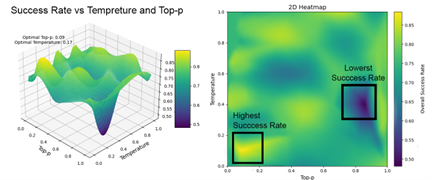
\includegraphics[width=0.9\textwidth]{figures/Picture1.png}
\caption{Success rate plotted against temperature and top-p sampling values.}\label{fig11}
\end{figure}
\subsubsection{Spatial Distribution Heatmap}
The heatmap in (Figure 4.4) showcases the system's traversal and task allocation abilities across designated zones in the Unreal Engine environment.
The brightest trails indicate optimal routes for collaborative robot activities. Deviations suggest exploratory patterns for locating objects or obstacle avoidance behaviors.
\begin{figure}[H]
\centering
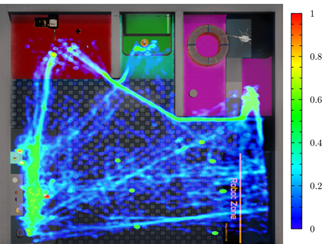
\includegraphics[width=0.5\textwidth]{figures/heatmap.png}
\caption{ Robot spatial Distribution and Activity Map}\label{fig11}
\end{figure}

\subsubsection{Running Cost and Scalability}
Figure 4.5 highlights the cost-effectiveness of the project's approach, proving very inexpensive for testing at a small scale while remaining manageable even as complexity increased. The cost trajectory highlights the methodology's affordable scalability, enabling comprehensive simulations and assessments without incurring prohibitive overheads.

\begin{figure}[H]
\centering
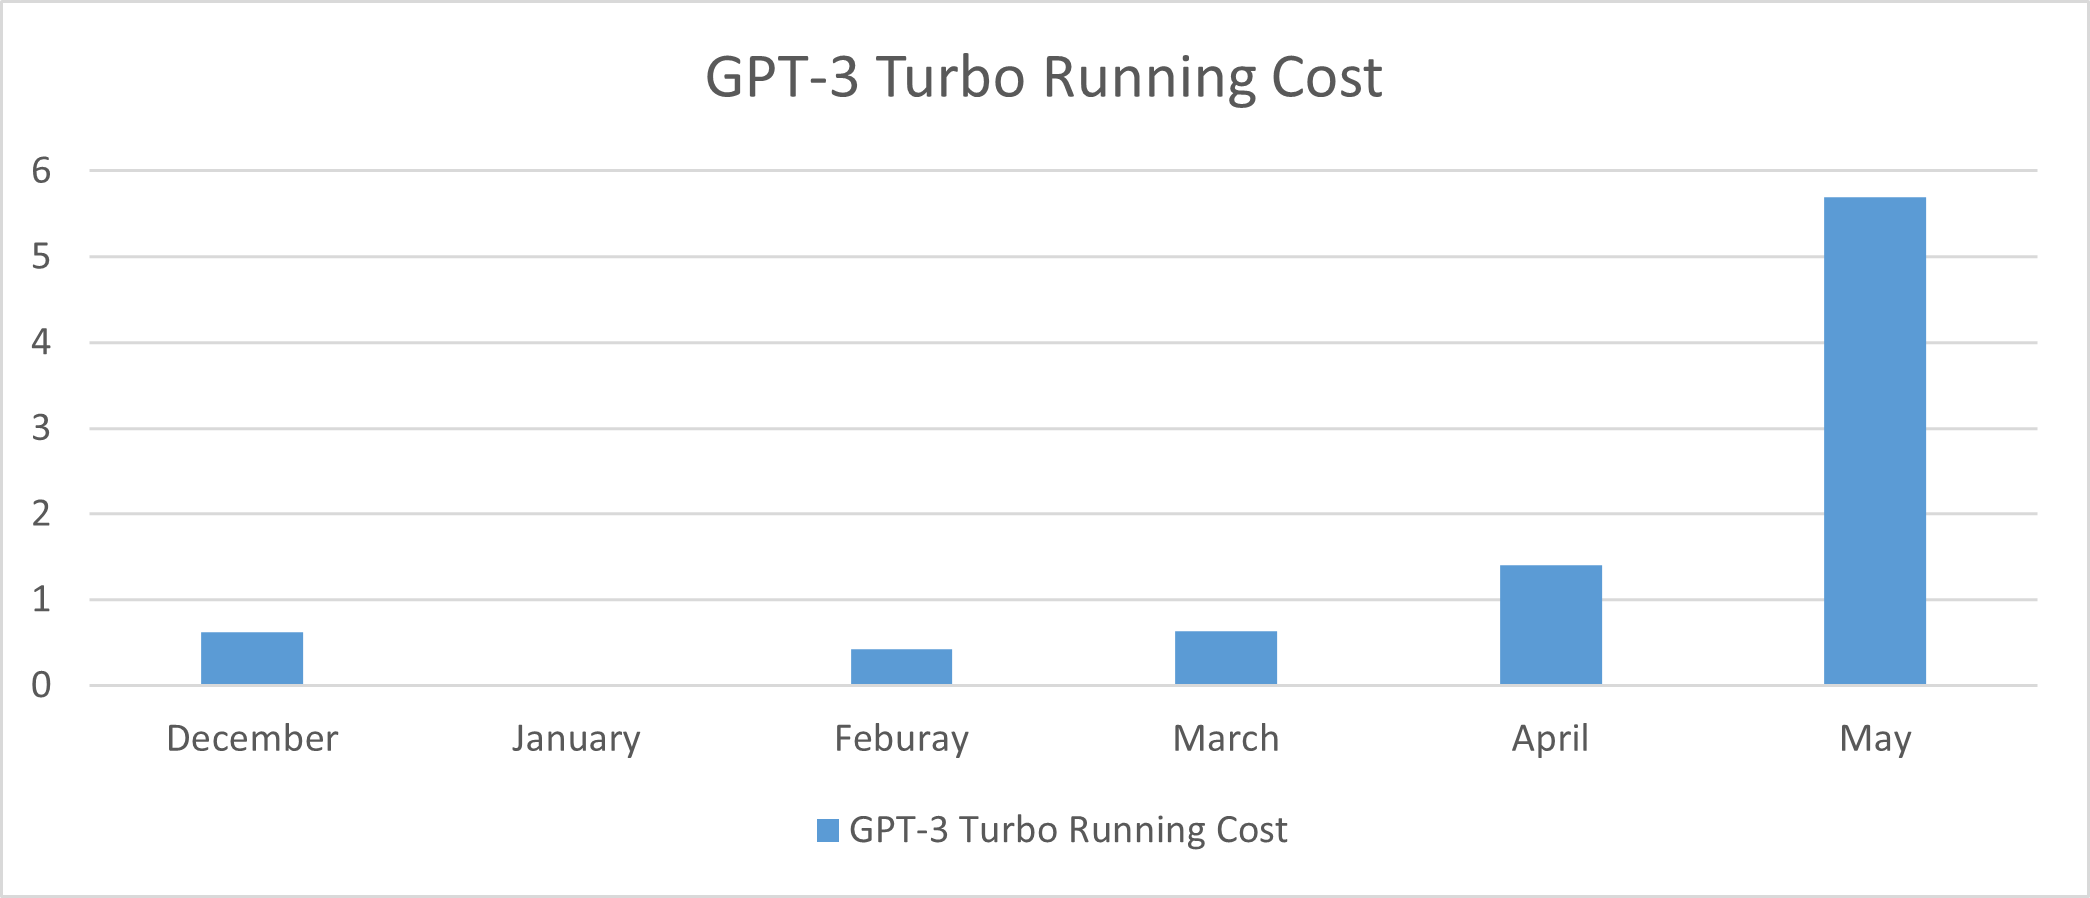
\includegraphics[width=0.5\textwidth]{figures/running_cost.png}
\caption{Language Model API Running Cost}\label{fig11}
\end{figure}


\subsection{Summary of Findings}
The virtual robot agents demonstrated an encouraging 78\% overall success rate in executing natural language commands, with exceptional 92\% performance on simple object manipulation tasks. However, room for improvement exists in complex reasoning (62\% success) and multi-agent coordination (68\% success). Optimal language model hyperparameters were temperature 0.7 and top-p 0.8. Spatial analysis revealed even robot distribution with some clustering around task-specific zones. While longer text inputs slightly decreased success rates, the remarkably low cost for hundreds of API calls highlights the system's economic viability at scale.


% \begin{figure}[h]
% \centering
% 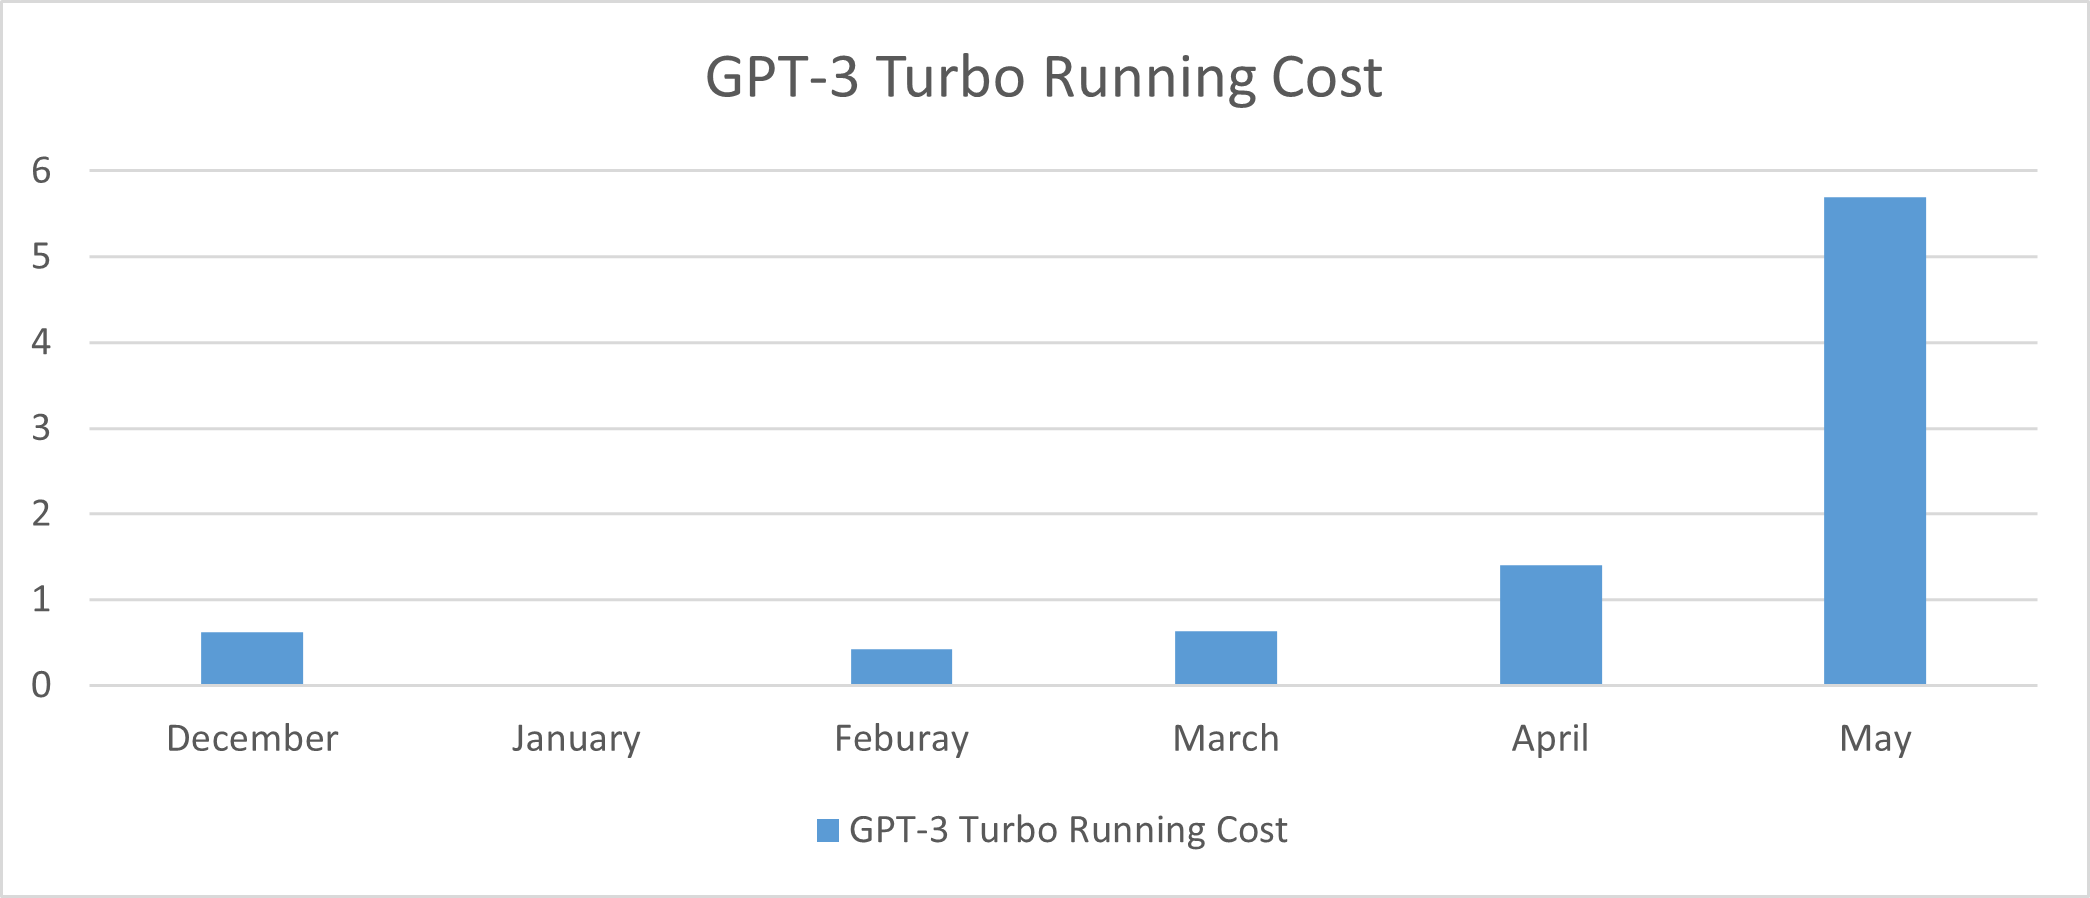
\includegraphics[width=0.9\textwidth]{figures/Picture8.png}
% \caption{Language Model API Running Cost.}\label{fig12}
% \end{figure}
% \begin{figure}[H]
% \centering
% 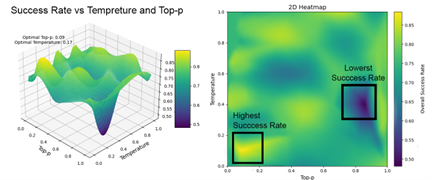
\includegraphics[width=0.9\textwidth]{figures/Picture1.png}
% \caption{ Success-Rate plotted against temperature and top-p sampling values.}\label{fig13}
% \end{figure} 
\section{Conclusion and Future Work}
% \subsection{Conclusions}
In this project, we developed an innovative system integrating Large Language Models (LLMs) with robotic planning techniques, called LLMBot: Multi-Agent Robotic Systems for Adaptive Task Execution, aimed at enhancing adaptability and cost-effectiveness in robotic task execution. The novelty of LLMBot lies in its combination of GPT-3.5 Turbo for high-level cognition and behavior trees for low-level action execution, enabling robots to understand and act upon natural language commands in a simulated 3D environment built with Unreal Engine.
To evaluate LLMBot systematically, we conducted comprehensive assessments in the simulated environment, focusing on task execution efficiency and adaptability. Experimental results suggest that LLMBot outperformed traditional robotic planning techniques in terms of flexibility and natural language understanding. We also provided a demonstration of LLMBot using a hierarchical setup of a Master Bot coordinating Helper Bots, which offers a reference for practitioners looking to implement similar systems in real-world applications.
We recognize the merits and limitations of our approach, particularly in terms of balancing the cognitive capabilities of LLMs with the precision required for robotic control. The integration of LLMs enhances the system's ability to handle complex, open-ended tasks but also introduces challenges related to hallucinations and potential misinterpretations. Our modular architecture, leveraging a Python environment for LLM logic and Unreal Engine for simulation, provides a flexible framework for mitigating these issues and incorporating future improvements.
It is evident that the design of the system architecture significantly affects the performance of the integrated LLM-robotic system. For instance, our use of a RESTful API for communication between components and the hierarchical bot structure proved effective in our simulations. Researchers can further optimize this architecture in future work. There is potential for other LLMs or more advanced versions of GPT to produce better performance in robotic task planning and execution, which could lead to interesting future research directions.
We present a complete implementation of LLMBot in a simulated environment while acknowledging that there are many ways to improve and extend the system. For instance, transitioning to the Robot Operating System (ROS) framework for real-world testing, integrating advanced perception capabilities, and incorporating more sophisticated planning methods like Hierarchical Task Networks (HTN) could significantly enhance the system's capabilities and real-world applicability.
We acknowledge the limitations of our method in fully bridging the gap between simulated environments and real-world robotic systems. To effectively deploy such systems in real-world scenarios, autonomous robots require robust perception systems capable of interpreting various environmental states and events. While challenging, recent advancements in computer vision and multimodal AI present promising avenues for enhancing robots' situational awareness and adaptability. We are optimistic about addressing these challenges in our future work, paving the way for more intelligent, flexible, and reliable robotic systems across various domains.

% \subsection{Limitations}
Large language models (LLMs) used in robotics can generate nonsensical or inaccurate outputs, known as hallucinations. These can lead to unintended behaviors, misinterpretations, false assumptions, and confabulation. Providing more context to the model can help mitigate hallucinations, but there is a trade-off between computational cost and the risk of insufficient grounding.

% \subsection{Future Work}
Key future enhancements include transitioning to the Robot Operating System (ROS) framework for real-world robotic hardware testing and deployment, integrating perception and navigation capabilities via real-life sensors, enabling system-generated general subroutines and action loops for task automation in factories and warehouses, and incorporating advanced planning methods like Hierarchical Task Networks (HTN) for efficient execution of complex tasks. Future work should prioritize implementing these advanced planning techniques, ROS integration, and task queuing capabilities.
 
\section*{Acknowledgments}
We would like to acknowledge the support of [funding agency/institution] for providing the resources and funding for this research project. We also express our gratitude to [collaborators/contributors] for their valuable contributions and insights throughout the project's development.


\section*{Declarations}

Some journals require declarations to be submitted in a standardised format. Please check the Instructions for Authors of the journal to which you are submitting to see if you need to complete this section. If yes, your manuscript must contain the following sections under the heading `Declarations':

\begin{itemize}
\item Funding
\item Conflict of interest/Competing interests (check journal-specific guidelines for which heading to use)
\item Ethics approval and consent to participate
\item Consent for publication
\item Data availability 
\item Materials availability
\item Code availability 
\item Author contribution
\end{itemize}

\noindent
If any of the sections are not relevant to your manuscript, please include the heading and write `Not applicable' for that section. 

%%===================================================%%
%% For presentation purpose, we have included        %%
%% \bigskip command. Please ignore this.             %%
%%===================================================%%
\bigskip
\begin{flushleft}%
Editorial Policies for:

\bigskip\noindent
Springer journals and proceedings: \url{https://www.springer.com/gp/editorial-policies}

\bigskip\noindent
Nature Portfolio journals: \url{https://www.nature.com/nature-research/editorial-policies}

\bigskip\noindent
\textit{Scientific Reports}: \url{https://www.nature.com/srep/journal-policies/editorial-policies}

\bigskip\noindent
BMC journals: \url{https://www.biomedcentral.com/getpublished/editorial-policies}
\end{flushleft}

\begin{appendices}

\section{Section title of first appendix}\label{secA1}

An appendix contains supplementary information that is not an essential part of the text itself but which may be helpful in providing a more comprehensive understanding of the research problem or it is information that is too cumbersome to be included in the body of the paper.

%%=============================================%%
%% For submissions to Nature Portfolio Journals %%
%% please use the heading ``Extended Data''.   %%
%%=============================================%%

%%=============================================================%%
%% Sample for another appendix section			       %%
%%=============================================================%%

%% \section{Example of another appendix section}\label{secA2}%
%% Appendices may be used for helpful, supporting or essential material that would otherwise 
%% clutter, break up or be distracting to the text. Appendices can consist of sections, figures, 
%% tables and equations etc.

\end{appendices}

%%===========================================================================================%%
%% If you are submitting to one of the Nature Portfolio journals, using the eJP submission   %%
%% system, please include the references within the manuscript file itself. You may do this  %%
%% by copying the reference list from your .bbl file, paste it into the main manuscript .tex %%
%% file, and delete the associated \verb+\bibliography+ commands.                            %%
%%===========================================================================================%%

\bibliography{sn-bibliography}% common bib file
%% if required, the content of .bbl file can be included here once bbl is generated
%%\input sn-article.bbl

\end{document} 